\documentclass[conference]{IEEEtran}
\usepackage[utf8]{inputenc}
\usepackage[T1]{fontenc}
\usepackage{lmodern}
\usepackage[english]{babel}
\usepackage{amsmath, amssymb, mathtools}
\usepackage{graphicx}
\usepackage{xcolor}
\usepackage{hyperref}
\usepackage{algorithm}
\usepackage[noend]{algpseudocode} % noend per non mostrare "end if", "end for", ecc.
\usepackage{booktabs} % Per linee di tabella più professionali
\usepackage{multirow} % Per celle che si estendono su più righe
\usepackage{siunitx}  % Per allineare i numeri per punto decimale e formattazione
\usepackage{enumitem} % Per personalizzare le liste
\usepackage{float}
\usepackage{placeins}
\usepackage{listings}
\usepackage{xcolor}
\usepackage{flushend} 
\usepackage{caption}
\pagenumbering{arabic}
\title{Toxicity, couple dynamics and most toxic sentence detection in Italian conversations using classical machine learning models and transformer-based models}

\author{
\IEEEauthorblockN{Davide Cirilli}
\IEEEauthorblockA{
Università degli Studi di Bari Aldo Moro \\
Email: d.cirilli2@studenti.uniba.it \\
Repo: \url{https://github.com/Davy592/NLP} }
}


\IEEEtitleabstractindextext{%
\begin{abstract}
This paper presents a comprehensive study on the detection of toxicity and personality-driven behaviors in Italian conversational data. We developed a system capable of classifying conversations as toxic or non-toxic, analyzing couple dynamics, and identifying or generating the most toxic sentences within a dialogue. Our approach combines traditional machine learning techniques, such as Logistic Regression and Naive Bayes, with advanced transformer-based models like BERT and BART. We evaluated these methods across different tasks, highlighting the strengths of fine-tuned transformer models in capturing subtle and complex patterns of toxicity. The system not only detects harmful interactions but also provides insights into personality-driven behaviors that may underlie toxic exchanges. To support practical use, we created a web application that offers a user-friendly interface for real-time toxicity detection, personality analysis, and the classification or generation of the most toxic sentence in a conversation. The study demonstrates the value of integrating classic and modern machine learning approaches to better understand and address toxic communication in digital spaces.
\end{abstract}
}%

\begin{document}
\maketitle
\IEEEdisplaynontitleabstractindextext

\section{Introduction and Motivations}

In today’s digital society, online platforms and social networks have become essential spaces for communication, shaping relationships and social interactions on a global scale. While these platforms offer numerous opportunities for connection and expression, they also create environments where toxic behaviors can spread, often with significant psychological and social consequences. This is especially true in conversations within intimate or emotionally charged contexts, where harmful behaviors may take the form of subtle manipulation, emotional control, or psychological abuse, rather than overtly offensive language.

Detecting and addressing such forms of toxicity is crucial for fostering safer and healthier digital environments. However, traditional approaches that focus on isolated messages or specific keywords often fall short in recognizing the complex dynamics that characterize toxic interactions. In particular, the interplay between conversational context and personality-driven behaviors demands more advanced tools capable of understanding deeper patterns of communication.

Our work aims to contribute to this challenge by exploring systems that combine toxicity detection with personality analysis, offering a more comprehensive view of harmful interactions in online dialogues. Beyond simply identifying toxic messages, these tasks play a vital role in supporting moderation efforts, promoting digital well-being, and informing interventions that can help prevent the escalation of harmful relationships in virtual spaces.

\section{Related Work}

The detection of toxicity and abusive language in online conversations has been widely explored, especially in English. Early approaches relied on machine learning classifiers such as SVM and Naive Bayes with hand-crafted features (e.g., n-grams, lexicons of offensive terms) to identify hate speech and offensive content \cite{AbusiveLanguageDetection2016} \cite{AutomatedHateSpeech2017}. More recent work leverages transformer-based models like BERT \cite{BERT2018} and RoBERTa \cite{RoBERTa2019}, showing significant improvements over traditional methods, particularly in capturing implicit and contextual toxicity \cite{HateSpeechDetectionSurvey2017}. Studies like \cite{ToxicityDetectionContext2021} highlight the importance of conversational context, noting that some messages are perceived as toxic only in relation to previous dialogue turns.

In the Italian language, projects such as EVALITA \cite{EVALITA2018} provided annotated datasets for hate speech detection, mostly focused on Twitter data. These efforts demonstrated the potential of both traditional models and fine-tuned multilingual transformers for Italian toxicity detection \cite{ResourcesBenchmarkHateSpeech2021}.

For personality detection, initial studies applied linguistic and psychological features (e.g., LIWC categories, stylistic markers) with classifiers like SVM to predict Big Five traits \cite{PersonalityRecognitionConversationText2007} \cite{WhoseThumb2006}. More recent approaches incorporate deep learning to infer personality traits from social media text \cite{PersonalityTraitDetectionBERT2020}. While many studies target English data, personality detection in Italian conversational data remains largely underexplored.

Our work extends this literature by addressing both toxicity and personality analysis simultaneously in Italian dialogues, leveraging transformer models to capture conversational context and personality-driven toxic behaviors in a unified system.

\section{Dataset preprocessing and Data augmentation}

In this section, we describe the dataset construction process, which involved integrating an existing toxic conversation dataset with a newly generated non-toxic conversation dataset. The goal was to create a balanced corpus that captures both toxic and healthy relationship dynamics in Italian conversations.

\subsection{Dataset preprocessing}

First of all, we applied a preprocessing step to the original dataset containing toxic conversations. The preprocessing steps were as follows:

\begin{itemize}
    \item \textbf{Standardization and cleaning:} We removed incomplete rows with missing names or conversation fields and excluded entries with irrelevant or malformed data. Names of participants were standardized to title case to ensure consistency.
    
    \item \textbf{Extraction of toxic sentences:} From the explanation field accompanying each conversation, we programmatically extracted the most toxic sentence using regular expressions.
    
    \item \textbf{Conversation reformatting:} We reformatted conversations using a hierarchical parsing logic. The system first tried to extract messages enclosed in quotation marks. If unavailable, it attempted to split the text using speaker labels (e.g., \texttt{Name:}) or speaker names. This aimed to segment and clean the dialogues effectively.
    
    \item \textbf{Final selection and export:} After cleaning, we retained the essential columns, including participant names, cleaned conversation, extracted toxic sentence, and explanation.
\end{itemize}

This structured preprocessing pipeline ensured that the data fed to our models was clean, consistently formatted, and suitable for both toxicity detection and personality analysis tasks.

\subsection{Dataset augmentation}

To enhance the dataset, we generated a complementary non-toxic conversation dataset using both Google's Gemini API and Google AI Studio. This automated generation process aimed to create realistic and culturally appropriate non-toxic dialogues in Italian, ensuring diversity in conversational patterns while adhering to safety guidelines.

\subsubsection{Automated generation with Gemini API}

The Gemini API was used to generate a large portion of the non-toxic conversation dataset. The model selected was \texttt{gemini-2.0-flash-lite}, configured with following parameters: 
\begin{itemize}
  \item \texttt{temperature} = 1.8: Promotes diverse and creative outputs by encouraging the model to explore a wider range of responses.
  \item \texttt{top\_p} = 1.0: Ensures all possible tokens are considered, avoiding restrictions on potential outputs.
  \item \texttt{top\_k} = 0: Disables top-k sampling, allowing unrestricted token sampling.
\end{itemize}
Strict safety settings were applied to block inappropriate content, with thresholds set to \texttt{BLOCK\_MEDIUM\_AND\_ABOVE} for all categories: harassment, hate speech, sexually explicit content, and dangerous content.

To guide generation, prompts specified role-based dynamics for each dialogue. The \texttt{person\_couple} classes used were:  
\begin{itemize}
    \item Insicuro e Supportivo
    \item Propositivo e Collaborativo
    \item Vulnerabile e Accogliente
    \item Pentito e Comprensivo
    \item Grato e Apprezzante
\end{itemize}
For each sample, a pair was selected randomly, and the API was instructed to generate a 6--10 turn dialogue reflecting the assigned dynamic, along with unique Italian names for the participants.  

Postprocessing involved parsing the raw response into structured fields: names, role pair, and dialogue. A custom parser extracted the names and cleaned each dialogue turn by removing speaker prefixes and ensuring proper punctuation and casing. Conversations not adhering to the required format (e.g., missing separator, insufficient turns, incomplete lines) were discarded. After generation, additional validation removed duplicates and normalized name casing, while ensuring that dialogue texts contained no residual formatting artifacts or repeated utterances.

\subsubsection{Generation with Google AI Studio}

Google AI Studio was used to complement the API-generated dataset, following the same parameter configuration as Gemini. The platform enabled batch generation with direct control over the response format. Each generated sample followed a predefined schema including:  
\begin{itemize}
    \item \texttt{person\_couple} class (randomly selected from the same list as above)
    \item two invented Italian names
    \item a complete, coherent dialogue
    \item \texttt{most\_toxic\_phrase} field always set to N/A
    \item \texttt{toxic} label fixed at 0
\end{itemize}
A key strength of this approach was the high structural consistency of the generated data, which minimized the need for parsing and reduced the risk of formatting errors. Furthermore, the output included explanations of why each conversation was classified as non-toxic, enhancing the dataset’s annotation richness.

\subsubsection{Postprocessing and integration}

Once generated, all data (from both sources) underwent additional processing. Conversations were checked for format consistency, proper turn alternation, and minimal length. Names were normalized (first letter uppercase, no trailing spaces), dialogues were cleaned of redundant whitespace, and duplicate conversations were removed.

At the end of this process, we had a comprehensive dataset containing around 950 toxic conversations and approximately 600 non-toxic conversations, each with detailed annotations.

\section{Approach}

In this section, we present our approach to toxicity detection, personality classification and most toxic sentence classification or generation in Italian conversational data. Our methodology integrates traditional machine learning techniques with advanced transformer-based models, specifically BERT and BART, to achieve robust performance across multiple tasks. The system is designed to handle both binary toxicity classification and personality-driven behavior analysis, providing a comprehensive solution for understanding toxic interactions in digital conversations.

\subsection{Binary Toxicity Classification}

\subsubsection{Without Text Preprocessing}

For the binary toxicity classification task, we first trained traditional machine learning models directly on raw conversational text. The dataset was split into training and test sets using an 80-20 stratified split to preserve class balance. We implemented two pipelines combining \texttt{TfidfVectorizer} with either Logistic Regression or Multinomial Naive Bayes classifiers. The \texttt{TfidfVectorizer} was configured with a bi-gram range (1,2).

Hyperparameter tuning was performed through grid search with 5-fold stratified cross-validation. For Logistic Regression, we optimized the regularization parameter \(C\) and the maximum number of features (3000, 5000, 7000). For Naive Bayes, we adjusted the smoothing parameter \(\alpha\) along with the number of features. The best configurations were selected based on weighted F1 measure.

\subsubsection{With Text Preprocessing}

To assess the impact of linguistic normalization, we applied additional preprocessing using the Italian \texttt{spaCy} model (\texttt{it\_core\_news\_sm}). Each conversation was lowercased, lemmatized, and stripped of stop words, punctuation, and spaces. The resulting text consisted of lemmatized content words, aiming to reduce noise and improve generalization.

We repeated the training and evaluation pipeline using these processed texts. The same classifiers and vectorization settings were used, although the grid search parameter space for max features was slightly reduced (2000, 4000, 6000) due to the more compact vocabulary after preprocessing.

\subsection{Couple Dynamics Prediction}

The couple dynamics prediction task aimed at classifying conversational excerpts according to the type of dyadic interaction, encoded in the \texttt{person\_couple} field of our dataset. Three distinct modeling strategies were explored: (i) a logistic regression model with Latent Semantic Analysis (LSA), (ii) logistic regression on frozen BERT embeddings, and (iii) a fine-tuned BERT model. Below we describe each method in detail.

\subsubsection{Logistic Regression with LSA}

We applied a pipeline consisting of TF-IDF vectorization, dimensionality reduction via Latent Semantic Analysis, and classification using logistic regression. The main components were:
\begin{itemize}
    \item \textbf{TF-IDF Vectorizer}: Extracted unigrams and bigrams to represent the conversations.
    \item \textbf{TruncatedSVD}: Reduced the feature space to latent topics, with the number of components optimized in \{100, 200, 300\}.
    \item \textbf{Logistic Regression}: Employed \texttt{lbfgs} solver and regularization parameter \(C \in \{0.1, 1, 10\}\).
\end{itemize}
Preprocessing was performed using the same spaCy pipeline as in the binary toxicity classification task, ensuring consistent text normalization. A grid search with 5-fold stratified cross-validation identified the best combination of latent components and regularization strength.

\subsubsection{Logistic Regression on Frozen BERT Embeddings}

In this variant, we leveraged the pre-trained Italian BERT model (\texttt{dbmdz/bert-base-italian-uncased}) without any fine-tuning. Each conversation was encoded as the \texttt{[CLS]} token embedding from BERT's last hidden layer:
\begin{itemize}
    \item \textbf{Tokenization}: Handled via \texttt{BertTokenizer} with truncation and padding to a maximum of 512 tokens.
    \item \textbf{Embedding Extraction}: The \texttt{last\_hidden\_state[:, 0, :]} vector was extracted for each sample.
\end{itemize}
These fixed-size embeddings served as input to a logistic regression classifier with \(C=0.1\) and maximum 2000 iterations. No additional text preprocessing was applied beyond BERT's built-in tokenization. This approach evaluated how well pre-trained contextual representations capture couple dynamics without task-specific adaptation.

\subsubsection{Fine-Tuned BERT}

The final method involved fine-tuning \texttt{dbmdz/bert-base-italian-uncased} directly on the classification task:
\begin{itemize}
    \item \textbf{Input Pipeline}: Used \texttt{BertTokenizer} with padding, truncation, and max length 512. Data was split into train, validation, and test sets (80/10/10 stratified).
    \item \textbf{Model}: Employed \texttt{BertForSequenceClassification} with label mappings derived from the \texttt{person\_couple} classes.
    \item \textbf{Training Configuration}: Set for up to 7 epochs, batch size 8, Adam optimizer with weight decay, and learning rate warmup. Early stopping with patience of 2 epochs was applied to prevent overfitting.
\end{itemize}
Post-training, we plotted loss curves to visualize learning dynamics and assessed the model on the test set via accuracy, classification report, and confusion matrix.

\subsubsection{Post-Processing and Analysis}

For all approaches, confusion matrices were generated to inspect misclassifications. Class labels were decoded using \texttt{LabelEncoder}, ensuring consistency across models. In the case of the BERT fine-tuned model, training and validation losses were additionally plotted to analyze convergence behavior. 

The classes considered in this task were all those present in the \texttt{person\_couple} field of the dataset (with both toxic and non-toxic conversations). The classes included:

\begin{itemize}
    \item Controllore E Isolata
    \item Dominante E Schiavo Emotivo
    \item Geloso-Ossessivo E Sottomessa
    \item Grato e Apprezzante
    \item Insicuro e Supportivo
    \item Manipolatore E Dipendente Emotiva
    \item Narcisista E Succube
    \item Pentito e Comprensivo
    \item Perfezionista Critico E Insicura Cronica
    \item Persona Violenta E Succube
    \item Propositivo e Collaborativo
    \item Psicopatico E Adulatrice
    \item Sadico-Crudele E Masochista
    \item Vittimista E Croccerossina
    \item Vulnerabile e Accogliente
\end{itemize}

This multi-model setup allowed us to compare traditional and transformer-based strategies in predicting conversational dynamics in Italian conversations.

\subsection{Most Toxic Sentence Detection}

The task of Most Toxic Phrase Detection focuses on identifying or generating the most toxic sentence within a conversation. We investigated two distinct approaches: (1) toxic phrase classification via fine-tuned BERT, and (2) toxic phrase generation using a BART-based seq2seq model.

\subsubsection{Most Toxic Phrase Classification with BERT}

For the classification approach, conversations were preprocessed to extract individual messages. Each message was paired with its corresponding couple identifier (as additional context) and labeled as toxic (1) if it matched the annotated most toxic sentence, or non-toxic (0) otherwise.

We employed the \texttt{dbmdz/bert-base-italian-uncased} model for fine-tuning. Inputs consisted of the message and couple identifier, tokenized using a maximum length of 128 tokens. The model was trained for up to 7 epochs with early stopping (patience = 2 epochs) based on validation loss. The training process used a batch size of 32, a learning rate of $2 \times 10^{-5}$, weight decay of 0.01, and the AdamW optimizer as implemented in Huggingface's \texttt{Trainer}. 

The dataset was stratified and split into 80\% training, 10\% validation, and 10\% test sets. Model evaluation on the test set involved computing accuracy, precision, recall, F1-score, and analyzing the confusion matrix.

At inference time, given a conversation, the model classifies each message independently and the one with the highest predicted probability of being toxic is selected as the most toxic sentence.

\subsubsection{Toxic Phrase Generation with BART}

In the generation-based approach, we framed the task as sequence-to-sequence learning: the input sequence consisted of the entire conversation (prefixed by a task descriptor), and the output was the annotated most toxic sentence. 

We used the \texttt{facebook/bart-base} model with a maximum input length of 512 tokens and output sequences truncated or padded to a maximum of 64 tokens.

The dataset was split using \texttt{GroupShuffleSplit} to ensure that train, validation, and test partitions (80\% / 10\% / 10\%) did not share structurally similar conversations, minimizing the risk of data leakage. Training employed early stopping (patience = 2 epochs), 7 epochs maximum, learning rate $3 \times 10^{-5}$, and a batch size of 4 due to memory constraints with large sequence inputs.

During inference, generation was performed using beam search (num\_beams = 4) with early stopping enabled. 

\subsection{Web Application for Real-Time Couple Dynamics and Most Toxic Phrase Detection}

To facilitate interactive experimentation and demonstration of the proposed models, we developed a web application using the \texttt{Gradio} framework. The application integrates three distinct transformer-based components: a couple dynamics classifier, a toxic sentence classifier, and a toxic sentence generator. 

\subsubsection{Architecture and Components}
\begin{itemize}
    \item \textbf{Couple dynamics prediction:} The application uses a fine-tuned BERT model (\texttt{dbmdz/bert-base-italian-uncased}) to classify the overall interaction pattern between two individuals based on their dialogue history. The classifier outputs one of 15 predefined relationship dynamics labels. The model produces class probabilities via a softmax layer, from which the most probable label and its confidence score are extracted.
    
    \item \textbf{Toxic sentence classification:} A second fine-tuned BERT model identifies the most toxic sentence within the conversation. Each message is encoded together with the predicted couple dynamics as context. The model assigns a toxicity probability to each message, and the sentence with the highest probability is selected.
    
    \item \textbf{Toxic sentence generation:} A fine-tuned BART model (\texttt{facebook/bart-base}) generates a toxic sentence summarizing the overall harmful content of the conversation. The model generates an output sequence using beam search decoding (4 beams, early stopping, maximum 64 tokens).
\end{itemize}

\subsubsection{Inference Workflow}
Users interact with the system by submitting individual chat messages. The application maintains conversation history and updates the couple dynamics prediction after each input. When requested, the application:
\begin{enumerate}
    \item Classifies the most toxic sentence by evaluating each message in the history.
    \item Generates a toxic sentence summarization using the BART model.
\end{enumerate}

\subsubsection{User Interface}
\noindent

\begin{figure}[H]
  \centering
  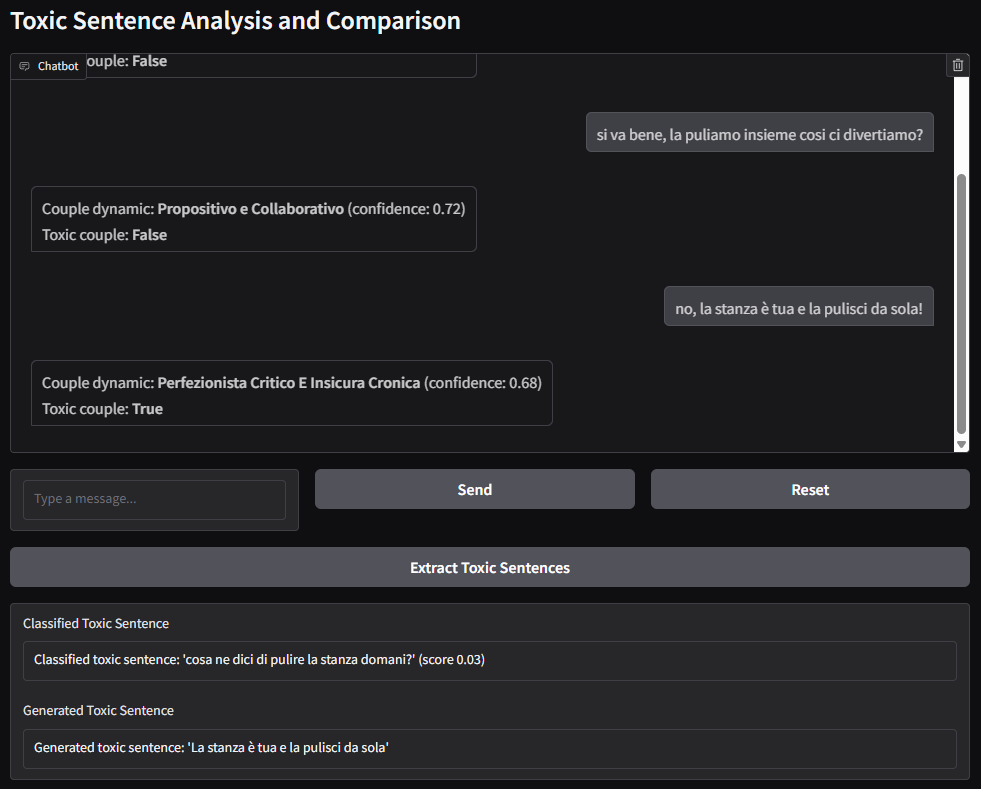
\includegraphics[width=\columnwidth]{figures/web_app_interface_used.png}
  \caption{Web application interface for couple dynamics and toxic sentence detection}
  \label{fig:web_app_interface}
\end{figure}

\subsubsection{Implementation Details}
Tokenization is performed dynamically at inference time. The BERT-based components use a maximum input length of 512 tokens (for couple dynamics) and 128 tokens (for toxic sentence classification), with appropriate truncation and padding strategies. The BART generator input is similarly truncated at 512 tokens to fit within the model's architecture limits.

The system provides both the predicted couple dynamics (including a binary toxic/not-toxic indication based on predefined labels) and the toxic sentence analyses, allowing direct comparison between classification-based and generation-based outputs.

\section{Results}

In this section, we present the results of our experiments on toxicity detection, couple dynamics prediction, and most toxic sentence detection.

\subsection{Binary Toxicity Classification}

The binary toxicity classification task was evaluated using two classical machine learning models: Logistic Regression and Multinomial Naive Bayes. Both were tested under two configurations: without text preprocessing, and with spaCy-based preprocessing (tokenization, lemmatization, stopword and punctuation removal).

\subsubsection{Hyperparameter Tuning}

\begin{itemize}
  \item \textbf{Without preprocessing:}
    \begin{itemize}
      \item \textbf{Logistic Regression:} $C = 10$, TF‑IDF max\_features = 3000.
      \item \textbf{Multinomial Naive Bayes:} $\alpha = 0.1$, TF‑IDF max\_features = 5000.
    \end{itemize}
  \item \textbf{With spaCy preprocessing:}
    \begin{itemize}
      \item \textbf{Logistic Regression:} $C = 10$, TF‑IDF max\_features = 2000.
      \item \textbf{Multinomial Naive Bayes:} $\alpha = 0.1$, TF‑IDF max\_features = 6000.
    \end{itemize}
\end{itemize}

\subsubsection{Performance Metrics}
\noindent

The models were evaluated on the test set using accuracy, precision, recall, and F1-score as metrics. The results are summarized in Table~\ref{tab:binary_classification_results}.

\begin{table}[H]
  \centering
  \begin{tabular}{lcccc}
    \toprule
    \textbf{Model} & \textbf{Accuracy} & \textbf{Precision} & \textbf{Recall} & \textbf{F1-score} \\
    \midrule
    Logistic Regression & 0.9968 & 0.9968 & 0.9968 & 0.9968 \\
    Multinomial NB      & 0.9968 & 0.9968 & 0.9968 & 0.9968 \\
    Log Reg (spaCy)     & 0.9936 & 0.9936 & 0.9936 & 0.9936 \\
    Multi NB (spaCy)    & 0.9968 & 0.9968 & 0.9968 & 0.9968 \\
    \bottomrule
  \end{tabular}
  \caption{Binary classification results with and without preprocessing}
  \label{tab:binary_classification_results}
\end{table}

\subsubsection{Confusion Matrices}
\noindent

Following there are the confusion matrices for each model configuration, which illustrate the classification performance in more detail.

\begin{figure}[H]
  \centering
  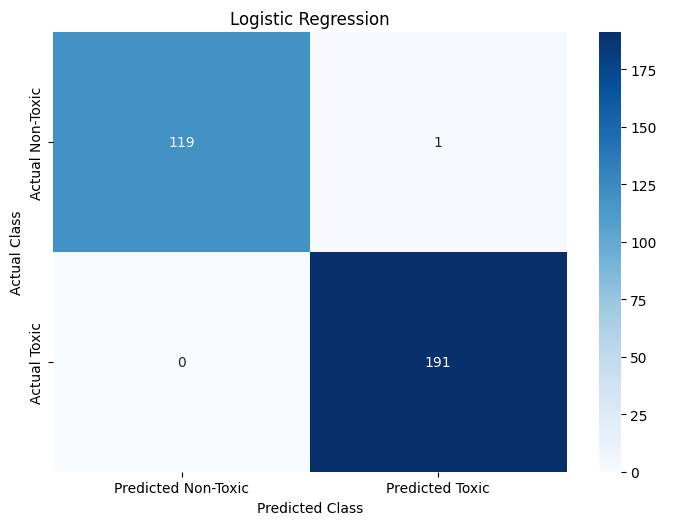
\includegraphics[width=0.9\columnwidth]{figures/confusion_lr_no_pre.png}
  \caption{Confusion matrix: Logistic Regression without preprocessing}
\end{figure}

\begin{figure}[H]
  \centering
  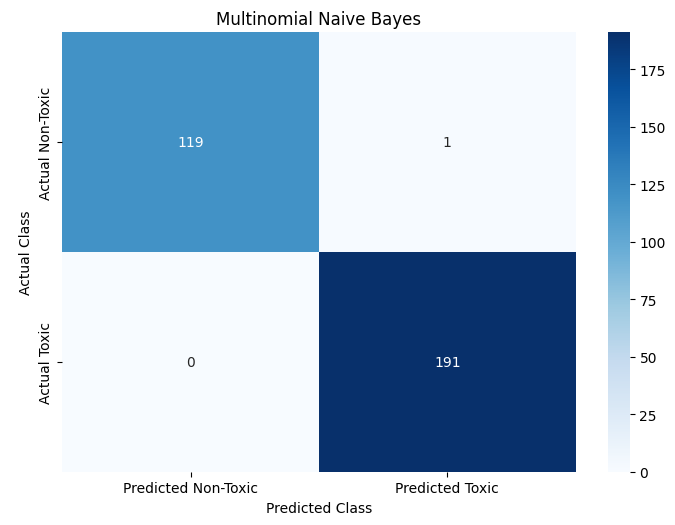
\includegraphics[width=0.9\columnwidth]{figures/confusion_nb_no_pre.png}
  \caption{Confusion matrix: Multinomial Naive Bayes without preprocessing}
\end{figure}

\begin{figure}[H]
  \centering
  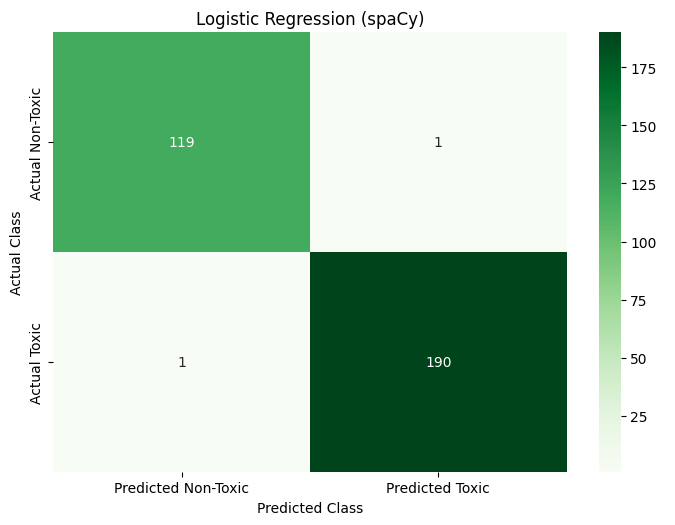
\includegraphics[width=0.9\columnwidth]{figures/confusion_lr_spacy.png}
  \caption{Confusion matrix: Logistic Regression with spaCy preprocessing}
\end{figure}

\begin{figure}[H]
  \centering
  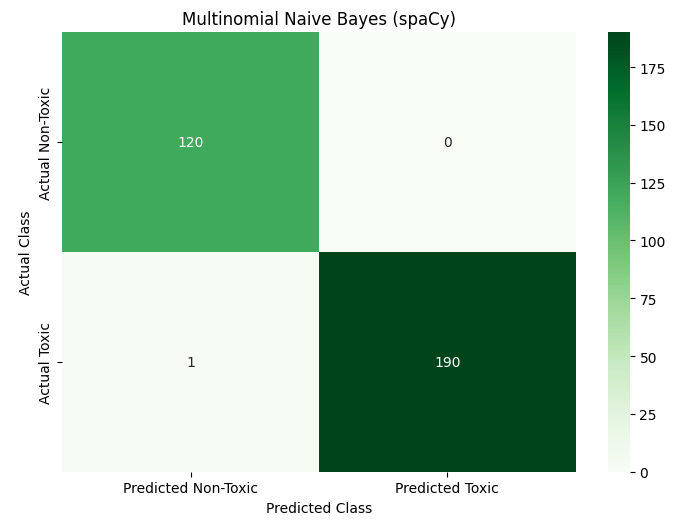
\includegraphics[width=0.9\columnwidth]{figures/confusion_nb_spacy.png}
  \caption{Confusion matrix: Multinomial Naive Bayes with spaCy preprocessing}
\end{figure}

\subsubsection{Discussion}

Both models achieved near-perfect performance, indicating strong separability between toxic and non-toxic samples. SpaCy preprocessing slightly reduced performance in logistic regression (from 0.9968 to 0.9936), likely due to the removal of informative lexical features. Multinomial Naive Bayes showed robustness across both configurations. These results suggest that simple ML models paired with TF‑IDF can be highly effective in this binary classification task when sufficient data is available.

\subsection{Couple Dynamics Prediction}

In this section, we compare the performance of three approaches applied to the couple dynamics prediction task: (i) LSA + Logistic Regression, (ii) BERT embeddings with Logistic Regression, and (iii) fine-tuned BERT.

\subsubsection{LSA + Logistic Regression}
\noindent
The LSA + Logistic Regression pipeline demonstrated reasonable performance, particularly excelling in classes with well-separated semantics (e.g., Grato e Apprezzante, Pentito e Comprensivo, Propositivo e Collaborativo). However, it struggled with more subtle or overlapping dynamics, such as Sadico-Crudele E Masochista and Geloso-Ossessivo E Sottomessa.

\begin{figure}[H]
  \centering
  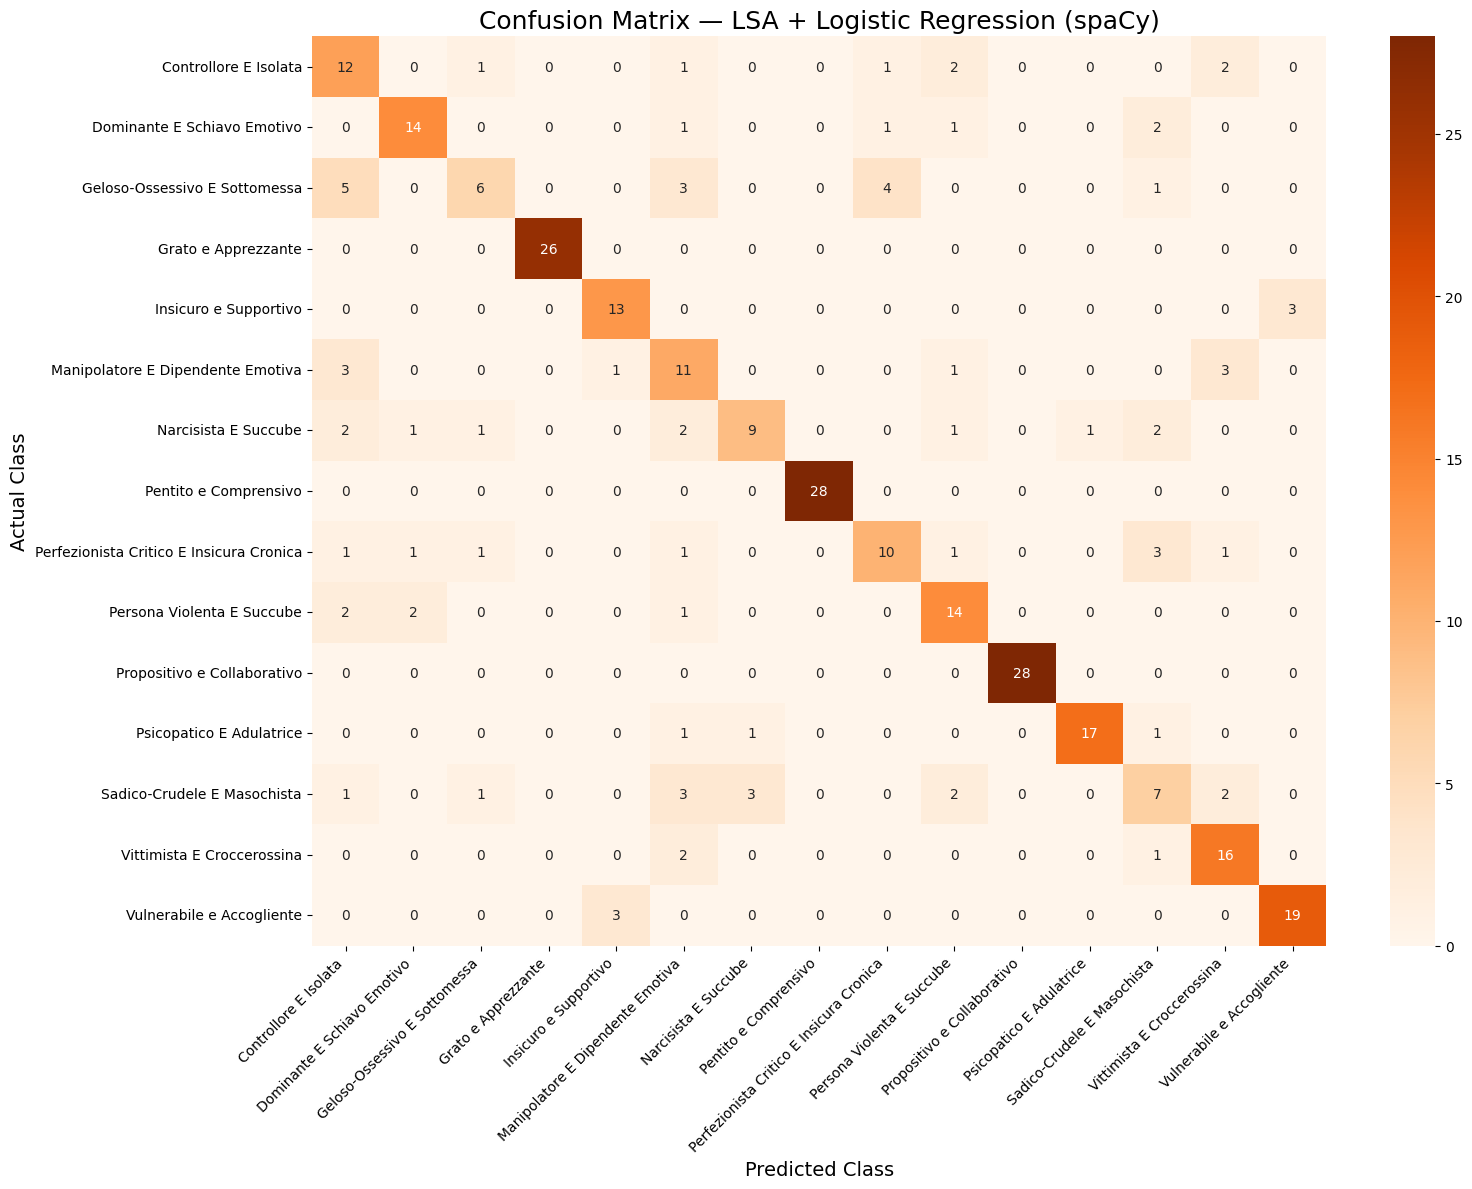
\includegraphics[width=\columnwidth]{figures/lsa_logreg_confusion_matrix.png}
  \caption{Confusion matrix for LSA + Logistic Regression}
\end{figure}

\vspace{1em}

\subsubsection{BERT Embeddings + Logistic Regression}
\noindent
Using pre-trained BERT embeddings as features yielded slightly lower performance compared to the LSA-based approach. While BERT embeddings capture richer semantics than LSA, the lack of task-specific fine-tuning likely limited their effectiveness in this multi-class setting. Some classes (Pentito e Comprensivo, Propositivo e Collaborativo) continued to be classified accurately, but the model struggled with more nuanced or less frequent dynamics.

\begin{figure}[H]
  \centering
  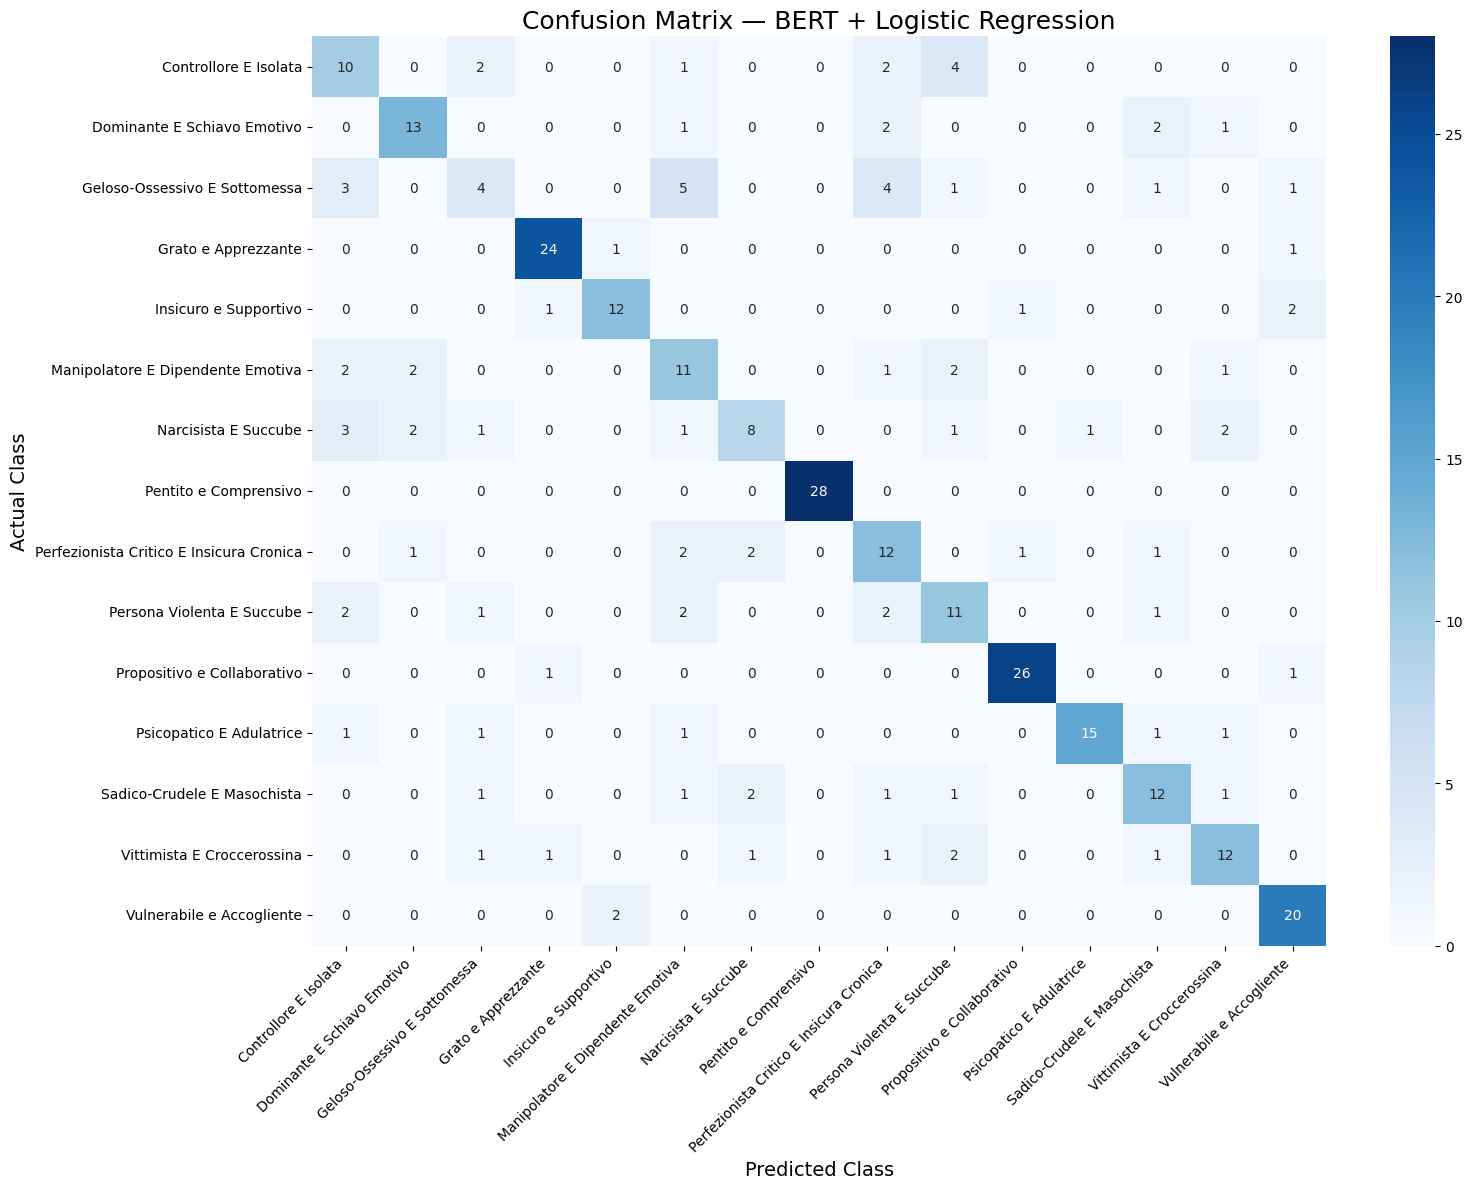
\includegraphics[width=\columnwidth]{figures/bert_logreg_confusion_matrix.png}
  \caption{Confusion matrix for BERT embeddings + Logistic Regression}
\end{figure}

\vspace{1em}

\subsubsection{Fine-tuned BERT}
\noindent
The fine-tuned BERT model outperformed both previous approaches. As depicted in the loss curves (Figure~\ref{fig:bert_loss}), the model exhibited good convergence behavior with no significant overfitting. The confusion matrix (Figure~\ref{fig:bert_cm}) further illustrates that this model provided more balanced predictions across most classes, including those that were difficult for previous approaches (e.g., Sadico-Crudele E Masochista, Vittimista E Croccerossina).

\begin{figure}[H]
  \centering
  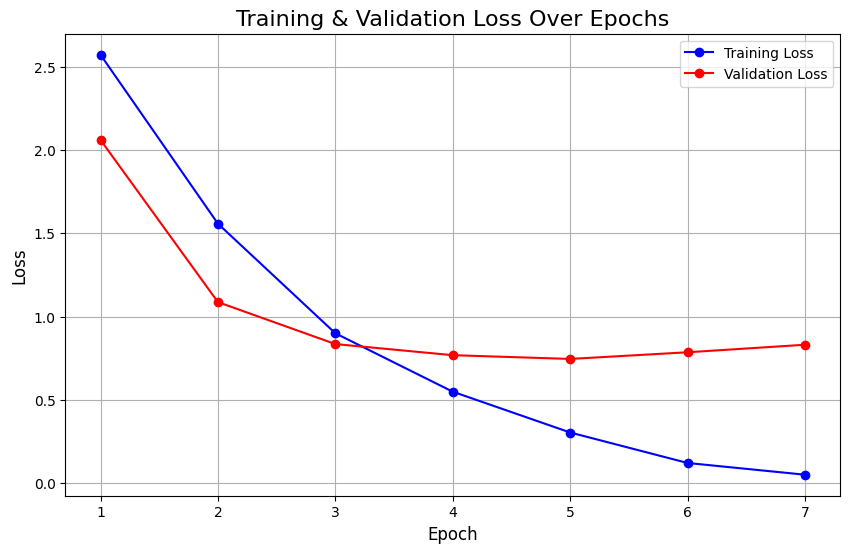
\includegraphics[width=\columnwidth]{figures/bert_finetuned_loss_curves.png}
  \caption{Training and validation loss curves for fine-tuned BERT}
  \label{fig:bert_loss}
\end{figure}

\begin{figure}[H]
  \centering
  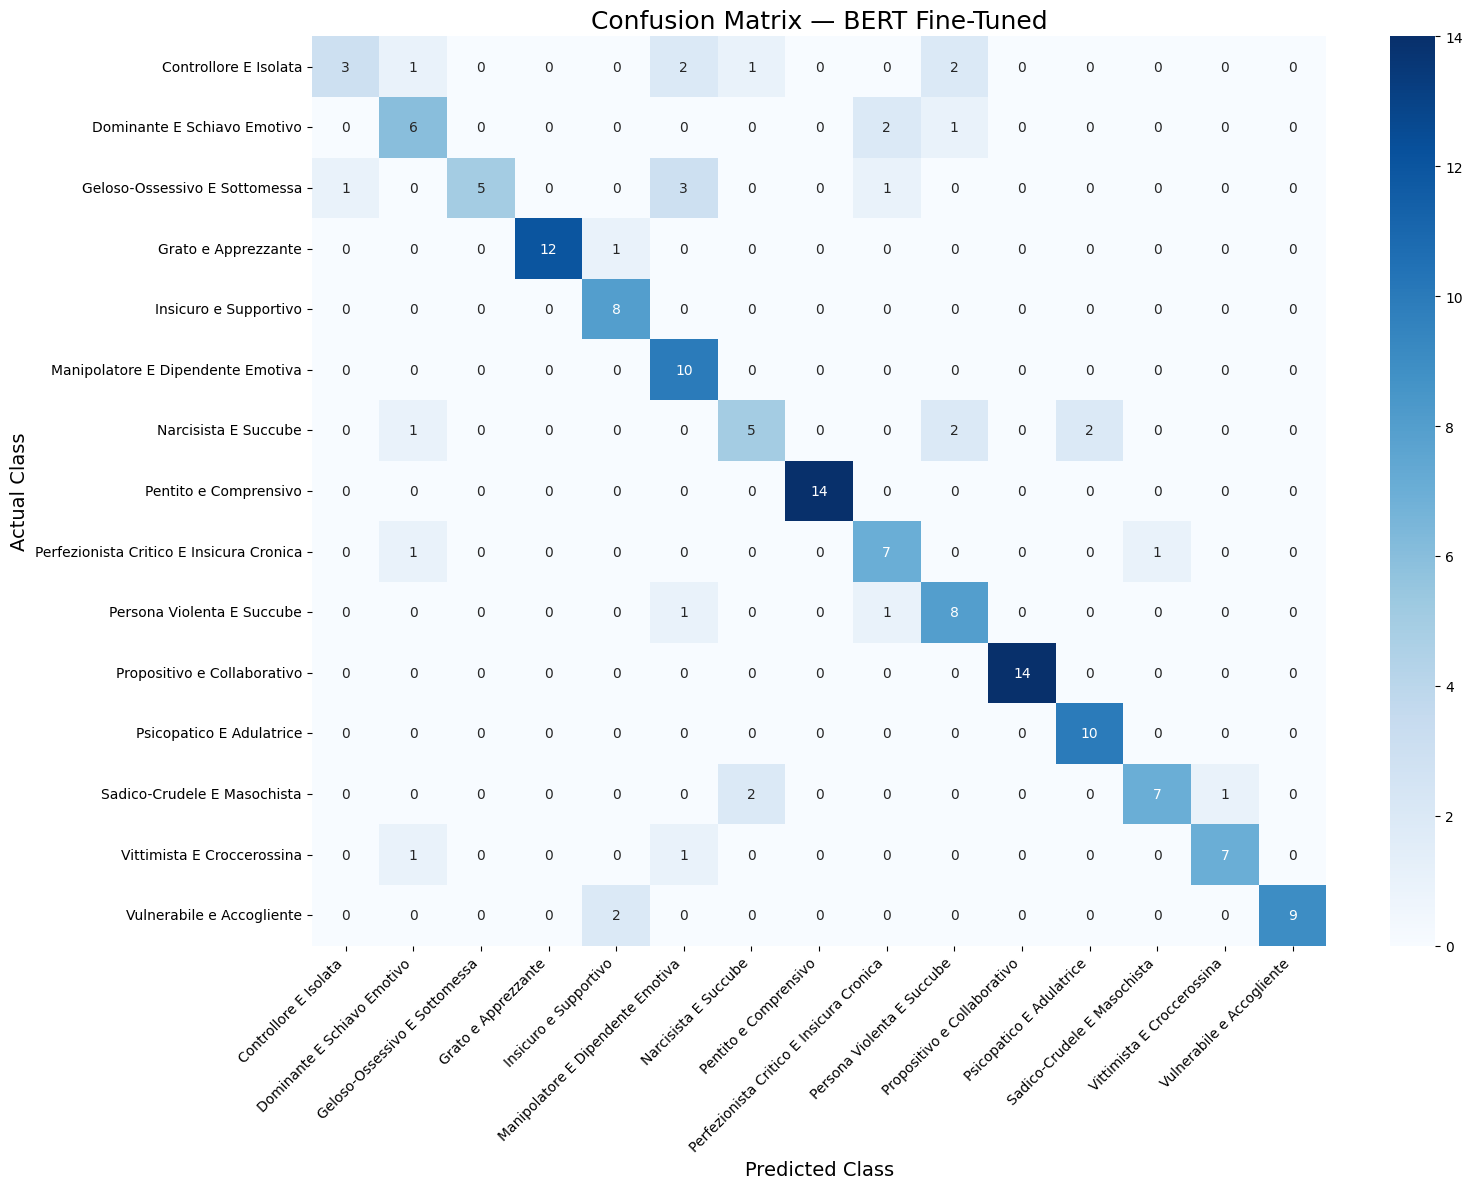
\includegraphics[width=\columnwidth]{figures/bert_finetuned_confusion_matrix.png}
  \caption{Confusion matrix for fine-tuned BERT}
  \label{fig:bert_cm}
\end{figure}

\vspace{1em}

\subsubsection{Summary of Results}
\noindent

Table~\ref{tab:all_results} provides a comparative summary of the test set performance for all models, with precision, recall, and F1-score reported as macro averages.

\begin{table}[H]
  \centering
  \begin{tabular}{lcccc}
    \toprule
    \textbf{Model} & \textbf{Accuracy} & \textbf{Precision} & \textbf{Recall} & \textbf{F1-score} \\
    \midrule
    LSA + Log Reg & 0.7363 & 0.7293 & 0.7133 & 0.7080 \\
    BERT + Log Reg & 0.7010 & 0.6840 & 0.6767 & 0.6753 \\
    Fine-tuned BERT & 0.8013 & 0.8093 & 0.7867 & 0.7780 \\
    \bottomrule
  \end{tabular}
  \caption{Comparison of model performance on the test set.}
  \label{tab:all_results}
\end{table}


\subsection{Most Toxic Sentence Detection}
\noindent

The most toxic sentence detection task was evaluated using two distinct approaches: (i) classification of sentences using a fine-tuned BERT model, and (ii) generation of toxic sentences using a BART-based seq2seq model. Below we present the results for each method.

\subsubsection{Most Toxic Sentence Classification with BERT}
\noindent

The BERT-based classifier achieved strong overall performance on the test set, as shown in Table~\ref{tab:bert_toxic_classification}. While the overall accuracy and weighted metrics are high, a detailed analysis reveals a significant imbalance in class-level performance. The classifier performed well for the Non-Toxic class, achieving high precision and recall, but struggled considerably with the Toxic class, yielding lower precision and recall. The low recall indicates that the model missed a large proportion of toxic phrases, likely due to the imbalance in the dataset where non-toxic sentences dominate. This suggests that despite fine-tuning, BERT had difficulty in detecting the minority class in a highly imbalanced setting.

\begin{table}[H]
  \centering
  \begin{tabular}{lcccc}
    \toprule
    \textbf{Class} & \textbf{Precision} & \textbf{Recall} & \textbf{F1-score} & \textbf{Support} \\
    \midrule
    Non-Toxic & 0.9077 & 0.9558 & 0.9311 & 679 \\
    Toxic & 0.3617 & 0.2048 & 0.2615 & 83 \\
    \midrule
    \textbf{Accuracy} & \multicolumn{4}{c}{0.8740} \\
    \textbf{Macro avg} & 0.6347 & 0.5803 & 0.5963 & 762 \\
    \textbf{Weighted avg} & 0.8482 & 0.8740 & 0.8582 & 762 \\
    \bottomrule
  \end{tabular}
  \caption{Performance metrics for BERT toxic phrase classification}
  \label{tab:bert_toxic_classification}
\end{table}

As depicted in the loss curves (Figure~\ref{fig:bert_loss_toxic}), the model initially achieved a good reduction in both training and validation loss. However, after the first few epochs, the validation loss began to increase while the training loss remained relatively stable, suggesting the onset of overfitting.

\begin{figure}[H]
  \centering
  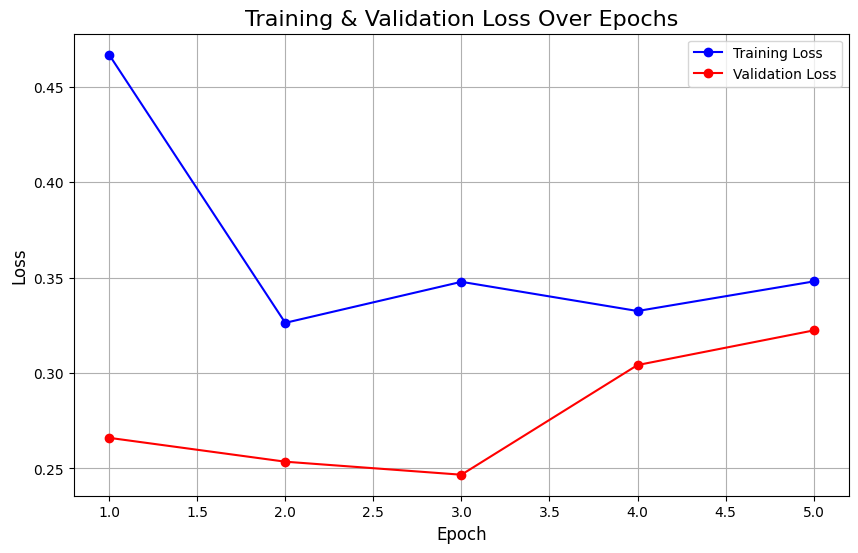
\includegraphics[width=\columnwidth]{figures/bert_toxic_loss_curves.png}
  \caption{Training and validation loss curves for BERT toxic phrase classification}
  \label{fig:bert_loss_toxic}
\end{figure}

\begin{figure}[H]
  \centering
  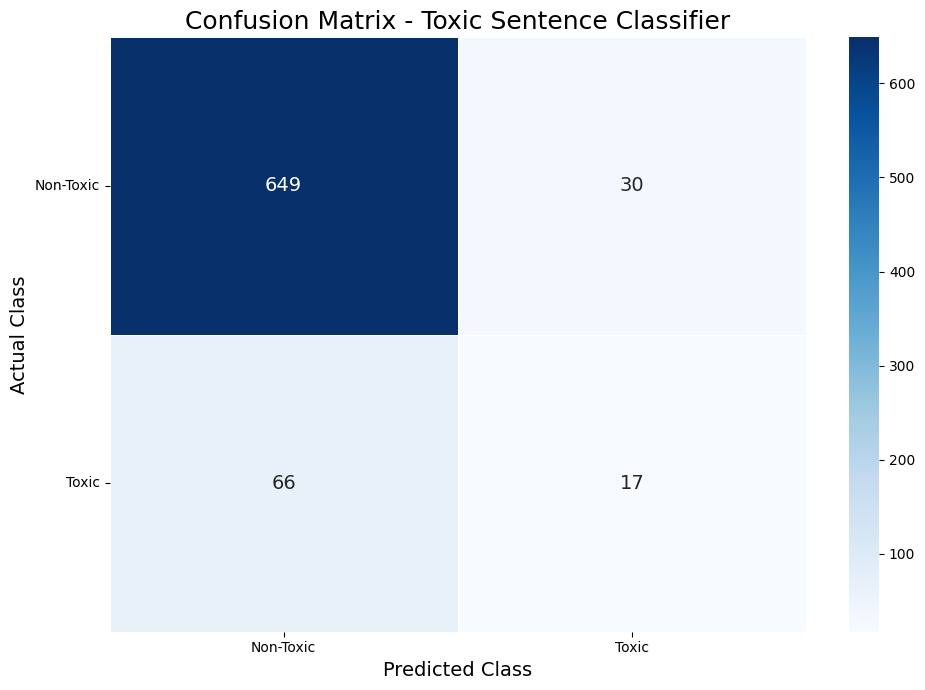
\includegraphics[width=\columnwidth]{figures/bert_toxic_confusion_matrix.png}
  \caption{Confusion matrix for BERT toxic phrase classification}
  \label{fig:bert_cm_toxic}
\end{figure}

\subsubsection{Most Toxic Sentence Generation with BART}
\noindent

For generation, we evaluated the BART model using BLEU and ROUGE metrics to assess the similarity between generated toxic phrases and human-labeled toxic phrases. 

\emph{BLEU} (Bilingual Evaluation Understudy) \cite{BLEU2002} measures the degree of n-gram overlap between the generated output and the reference text. Specifically, it computes precision over n-grams (where $n=1,2,\dots$), penalized by a brevity penalty to discourage overly short outputs. In this work, we computed sentence-level BLEU scores with smoothing to mitigate the problem of zero scores when no n-gram matches are found in short sentences.

\emph{ROUGE} (Recall-Oriented Understudy for Gisting Evaluation) \cite{ROUGE2004} is a suite of metrics designed to evaluate text summarization and generation quality. We report three commonly used ROUGE variants:
\begin{itemize}
    \item \textbf{ROUGE-1:} Measures the overlap of unigrams (individual words) between the generated and reference sentence. It reflects how many words of the reference are captured by the output.
    \item \textbf{ROUGE-2:} Measures the overlap of bigrams (sequences of two consecutive words). This provides a stronger indication of fluency and local coherence.
    \item \textbf{ROUGE-L:} Based on the longest common subsequence (LCS), this metric captures the extent to which the generated output preserves the sequence and order of words found in the reference.
\end{itemize}
For ROUGE, we reported the \emph{F1} measure, which balances precision and recall at the n-gram level.

All metrics were averaged over the test set to provide a global estimate of model performance. The use of both BLEU and ROUGE allowed us to evaluate the generated text along complementary dimensions: BLEU focusing more on precision of n-gram matches, and ROUGE emphasizing recall and sequence fidelity.

The results achieved by the model are shown in Table~\ref{tab:bart_toxic_generation}. These results suggest that the generated phrases exhibit some lexical overlap with the reference toxic phrases; however, the relatively low scores highlight the difficulty of producing exact matches in open-ended, linguistically diverse tasks such as toxic phrase generation. The metrics indicate that BART was able to capture certain key n-grams and longer subsequences from the reference phrases, though there is still considerable room for improvement in terms of fluency and semantic alignment.

\begin{table}[H]
  \centering
  \begin{tabular}{lc}
    \toprule
    \textbf{Metric} & \textbf{Score} \\
    \midrule
    BLEU & 0.1706 \\
    ROUGE-1 & 0.3031 \\
    ROUGE-2 & 0.2170 \\
    ROUGE-L & 0.2987 \\
    \bottomrule
  \end{tabular}
  \caption{Performance metrics for BART toxic phrase generation}
  \label{tab:bart_toxic_generation}
\end{table}

As seen in the loss curves (Figure~\ref{fig:bart_loss_toxic}), the model's training dynamics show a steady decrease in training loss across epochs, while the validation loss remains low and relatively stable. This indicates that the model fits the training data progressively better without significant overfitting.

\begin{figure}[H]
  \centering
  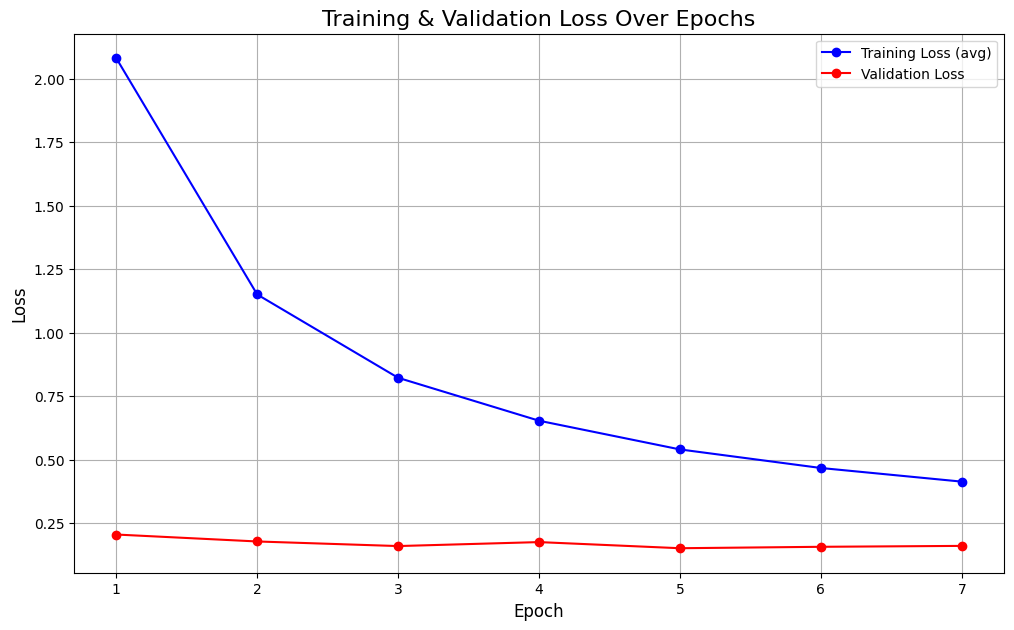
\includegraphics[width=\columnwidth]{figures/bart_toxic_loss_curves.png}
  \caption{Training and validation loss curves for BART toxic phrase generation}
  \label{fig:bart_loss_toxic}
\end{figure}

\section{Conclusion}

In this report, we presented a comprehensive approach to toxicity detection, couple dynamics analysis and most toxic sentence detection in Italian conversational data. Our methodology combined traditional machine learning techniques with advanced transformer-based models, specifically BERT and BART, to achieve robust performance across multiple tasks.

We successfully generated a synthetic dataset of Italian conversations, which was used to train and evaluate our models. The binary toxicity classification task demonstrated that classical machine learning models, such as Logistic Regression and Multinomial Naive Bayes, can achieve nearly perfect accuracy even without extensive text preprocessing.

The couple dynamics prediction task highlighted the effectiveness of fine-tuned BERT models in capturing complex relational patterns, achieving an accuracy of 80.13\%.

The most toxic sentence detection task showcased the strengths and limitations of both classification and generation approaches. The BERT-based classifier achieved high accuracy but struggled with class imbalance, while the BART generator produced reasonable toxic phrases with some lexical overlap to human-labeled references.

Finally, we developed a web application using the Gradio framework to facilitate interactive experimentation and demonstration of our models. This application allows users to explore couple dynamics and toxic sentence detection in real-time, providing a user-friendly interface for understanding conversational toxicity.

\section{Limitations and Future Work}

\subsection{Current Limitations}

While our approach has demonstrated promising results, several limitations remain:

\begin{itemize}
    \item \textbf{Class Imbalance:} The binary toxicity classification and most toxic sentence detection tasks faced significant class imbalance, which affected model performance. Future work should explore techniques such as oversampling, undersampling, or using focal loss to mitigate this issue.
    \item \textbf{Interpretability:} The black-box nature of transformer models makes it challenging to interpret their decisions. Future work should explore techniques for model interpretability to better understand the factors driving toxicity predictions.
    \item \textbf{Real-time Performance:} The web application, while functional, may face performance issues with larger conversations or more complex models. Future work should optimize the inference pipeline and consider model distillation or quantization techniques to improve real-time responsiveness.
\end{itemize}

\subsection{Future Directions}

Future work could explore the following directions:

\begin{itemize}
    \item \textbf{Use of different loss functions:} Experimenting with different loss functions, such as focal loss or label smoothing, to address class imbalance and improve model performance on minority classes.
    \item \textbf{Pairwise training and tournament evaluation:} Adopting a pairwise training approach for BERT models to learn comparative toxicity relationships, such as "A is more toxic than B". This could be assessed using a tournament-style evaluation, where models compare pairs of conversations to derive more refined insights into couple dynamics.
    \item \textbf{Adding explanations to predictions:} Enhancing the web application to provide explanations for toxicity predictions, such as highlighting specific phrases or words contributing to the classification.
    \item \textbf{Expanding the dataset:} Collecting more diverse conversational data to improve model generalization and robustness, particularly for underrepresented classes in couple dynamics.
    \item \textbf{Exploring other transformer architectures:} Investigating alternative transformer models, such as RoBERTa or GPT, to compare their performance on toxicity detection and couple dynamics analysis.
    \item \textbf{Incorporating user feedback:} Implementing a feedback loop in the web application to allow users to provide corrections or additional context, which could be used to iteratively improve model performance.
\end{itemize}
\noindent

\bibliographystyle{IEEEtran}
\bibliography{bibliografia}
\end{document}